\documentclass[pdftex,12pt,a4paper]{report}

\usepackage[portuguese,english]{babel}
\usepackage[T1]{fontenc} 
\usepackage[table]{xcolor}
\usepackage[utf8]{inputenc}
\usepackage[pdftex]{graphicx}
\usepackage{minitoc}
\usepackage{hyperref}
\usepackage{indentfirst}
\usepackage[compact]{titlesec}
\usepackage{fancyhdr}
\usepackage{caption}
\usepackage{pgfplots}
\usepackage{pgfplotstable}
\usepackage{fixltx2e}
\usepackage{mathtools}
\usepackage{fancyhdr}
\usepackage{listings}
\usepackage{color}
\usepackage{sverb}
\usepackage[section]{placeins}
%Highlight
\newcommand{\shellcmd}[1]{\\\indent\indent\texttt{\footnotesize\# #1}\\}

\pagestyle{fancy}
\renewcommand*\thesection{\thechapter\arabic{section}}
\newcommand{\HRule}{\rule{\linewidth}{0.5mm}}
\begin{document}

\begin{titlepage}

\begin{center}


\includegraphics[width=0.15\textwidth]{./logo}\\[0.5cm]    

\textsc{\large Universidade de Aveiro \\[1cm]\large departamento de electrónica, telecomunicações e informática}\\[1cm]

\textsc{\large{47022}\large - Arquitectura de Computadores Avançada \\[1cm]}

\HRule \\[0.5cm]
{ \huge \bfseries  Home group assignment 1}\\[0.4cm]
{ \large \bfseries Implementing a forwarding and stall unit in a pipelined architecture}\\[0.4cm]
\HRule \\[1cm]

\textsc{\small{8240 - MESTRADO INTEGRADO EM ENGENHARIA DE COMPUTADORES E TELEMÁTICA}}\\[1cm]

\begin{minipage}{0.4\textwidth}

\begin{flushleft} \large
\href{mailto:rafael.ferreira@ua.pt}{António Rafael da \\ Costa Ferreira }
 \small{\\NMec: 67405 | P4G1}
\end{flushleft}
\end{minipage}
\begin{minipage}{0.4\textwidth}

\begin{flushright} \large
\href{mailto:rodrigocunha@ua.pt}{Rodrigo Lopes \\ da Cunha}
\small{\\NMec: 67800 | P4G1}
\end{flushright}
\end{minipage}\\[1cm]

{\large Docentes: Nuno Lau/José Luís Azevedo   }\\[0.5cm]

\vfill

{\large Novembro de 2015 \\ 2015-2016}

\end{center}

\end{titlepage} %Titulo do Relatorio
\renewcommand{\headrulewidth}{0pt}

%Cabeçalhos de rodapé
\fancyhead{}
\fancyfoot{}
\lhead{Home group assignment 2}
\rhead{ACA - 2015/2016}
\lfoot{Rafael Ferreira nmec: 67405 \\ Rodrigo Cunha nmec: 67800}
\rfoot{\thepage}

%Renomear Comandos
\renewcommand*\contentsname{Conteúdos}
\renewcommand*\figurename{Figura}
\renewcommand*\tablename{Tabela}

%Conteúdos, dar paragrafo
\tableofcontents
%Headers
\renewcommand{\headrulewidth}{0.15pt}
\renewcommand{\thechapter}{}

\clearpage

\section{Introdução}
% o que, porquê e o objetivo

O trabalho proposto para a unidade curricular de Arquitetura de Computadores Avançada foi a implementação em CUDA para o processamento de um Semi-Global Matching. 

Este programa tem como objetivo determinar a imagem de disparidade entre duas imagens idênticas mas de posições diferentes, como se de dois olhos se tratasse, uma vista com o olho da esquerda e outra com o olho da direita.

O relatório reflete todas as geometrias de kernel implementadas, formas de pensamento, métodos de como foram implementados os algoritmos, resultados, tutorial para correr o código elaborado, e por último a conclusão deste mesmo trabalho.

\newpage
\section{Exercício 1}

\subsection{Cuda Kernel da função "determine\_costs()"}
Neste primeiro exercício, era pedido que se desenvolvesse um kernel em CUDA que substituísse a função \textit{determine\_costs()}.

\begin{figure}[!htb]
\center
 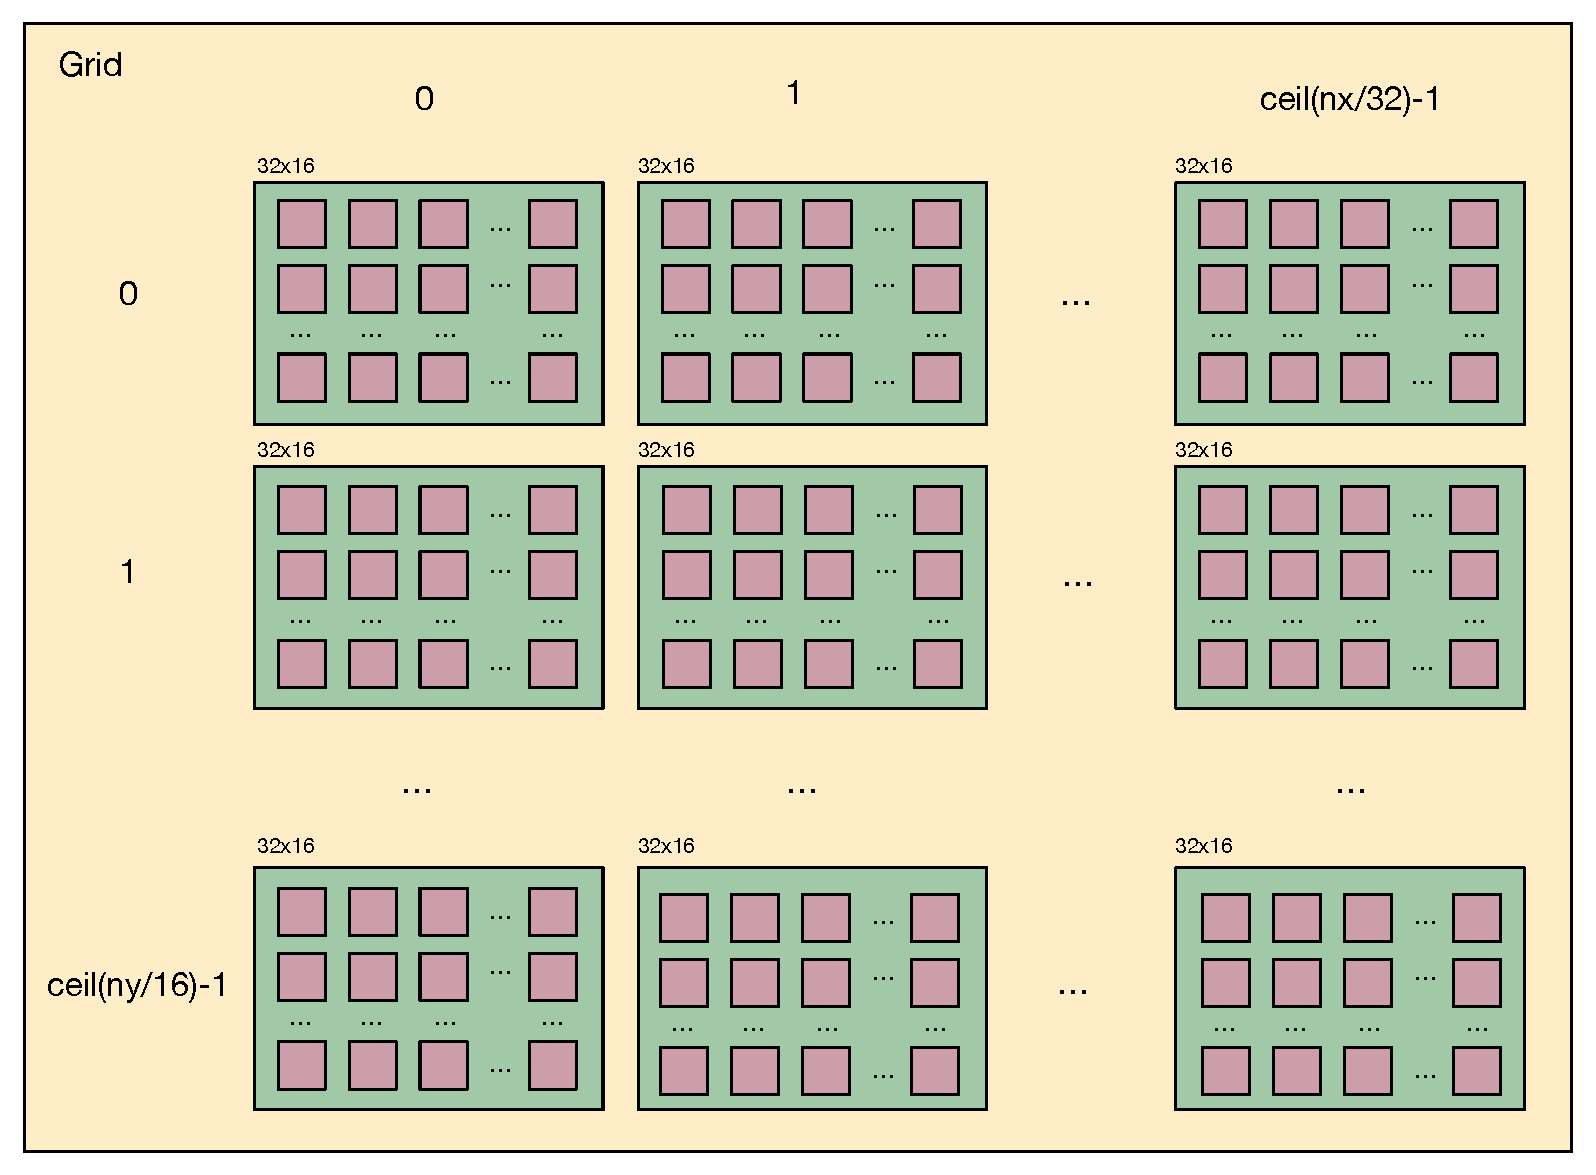
\includegraphics[width=100mm,scale=1]{DetermineCosts_v1_kernel.pdf}
 \caption{\\ Geometria do Kernel para a função determine\_costs()}
 \label{fig:DetermineCosts_v1_kernel}
\end{figure}

Neste kernel optou-se por uma geometria (Figura \ref{fig:DetermineCosts_v1_kernel}  constituída por uma grid de tamanho (ceil(nx\/32) x ceil(ny\/16)) com blocos de 32 x 16 threads cada.
Nesta função, cada thread corresponde a um pixel da imagem, e cada um calcula o valor de custo, sendo este a diferença entre as imagens num determinado pixel.

Este exercicío foi ainda realizado de duas maneira, uma utilizando a \textit{global memory}, e outra onde se coloca as imagens e o valor de COSTS na \textit{texture memory}. 

Para a \textit{global memory} utilizou-se o seguinte algoritmo para desenvolver o kernel:

\begin{lstlisting}[language=c++, basicstyle=\scriptsize]
__global__ void determine_costs_device(const int *left_image,  const int *right_image,
 int *costs, 
const int nx, const int ny, const int disp_range)
{
  int i = blockIdx.x * blockDim.x + threadIdx.x;
  int j = blockIdx.y * blockDim.y + threadIdx.y;

  if (i < nx && j < ny)
  {
    for ( int d = 0; d < disp_range; d++ ) {
      if(i >= d){
        COSTS(i,j,d) = abs( LEFT_IMAGE(i,j) - RIGHT_IMAGE(i-d,j));
      }
    }
  }
}
\end{lstlisting} 

Com esta implementação obtiveram-se os seguintes resultados:

\begin{figure}[!htb]
\center
 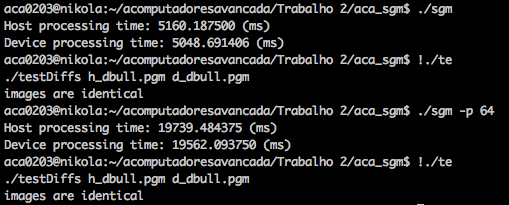
\includegraphics[width=100mm,scale=1]{DetermineCostsv1globalresults.png}
 \caption{\\ Resultados obtidos utilizando global memory}
 \label{fig:DetermineCostsv1globalresults}
\end{figure}


TEXTURE MEMORY CODIGO E RESULTADOS

\newpage
\section{Exercício 2}

\subsection{Cuda Kernel(s) da função "iterate\_direction\_dirxpos\_dev()" e das funções correspondestes a outras direcções}

Para este exercicío foram implementadas duas versões para a utilização de \textit{global memory}, sendo a versão 2 (otimizada) utilizada na utilização da \textit{shared memory}.

\subsubsection{Versão 1}

Nesta versão, foram criadas duas geometrias apenas, sendo que uma diz respeito às iterações nas direções em x, e outra em y, visto que tanto para o lado positivo como para o negativo a geometria era idêntica.

 \begin{figure}[!htb]
\center
 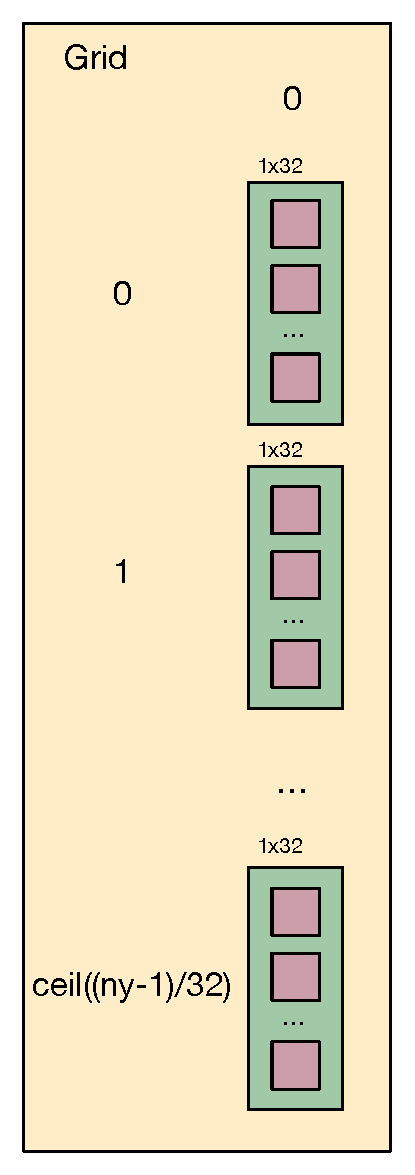
\includegraphics[width=100mm,scale=1]{IteratePositionDirxposneg_v1_kernel.pdf}
 \caption{\\ Geometria do Kernel para as funções iterate\_position\_dirxpos() e iterate\_position\_dirxneg()}
 \label{fig:IteratePositionDirxposneg_v1_kernel}
\end{figure}

Como podemos ver na figura \ref{fig:IteratePositionDirxposneg_v1_kernel}, a grid é composta por ny blocos, 

\newpage
\section{Conclusão}

Este trabalho foi útil para assentar todos os conhecimentos que se foi obtendo ao longo destes anos, tanto em Arquitectura de Computadores Avançada como em Arquitetura de Computadores I e II. Ambas as entregas foram primeiro planeadas em papel antes de se avançar para a implementação o que resultou em bons resultados a nível de tempo despendido, para ambos as entregas fez-se uso de dois dias de trabalho.

Na primeira entrega houve uma falha na implementação, esqueceu-se de realizar o shift left 2 do program counter para calcular o endereço para onde é suposto saltar a instrução jump.

Já na segunda entrega teve-se os máximos cuidados para que tudo funcionasse perfeitamente.

\end{document}